\documentclass[a4paper,11pt]{article}
\input{/home/tof/Documents/Cozy/latex-include/preambule_doc.tex}
\input{/home/tof/Documents/Cozy/latex-include/preambule_commun.tex}
%\newcommand{\showprof}{show them}  % comment this line if you don't want to see todo environment
\setlength{\fboxrule}{0.8pt}
\fancyhead[L]{\fbox{\Large{\textbf{DonRep 01}}}}
\fancyhead[C]{\textbf{Représentation des entiers naturels}}
\newdate{madate}{10}{09}{2020}
%\fancyhead[R]{\displaydate{madate}} %\today
\fancyhead[R]{Première - NSI}
\fancyfoot[L]{\vspace{1mm}Christophe Viroulaud}
\AtEndDocument{\label{lastpage}}
\fancyfoot[C]{\textbf{Page \thepage/\pageref{lastpage}}}
\fancyfoot[R]{\includegraphics[width=2cm,align=t]{/home/tof/Documents/Cozy/latex-include/cc.png}}
\usepackage{tikz}
\begin{document}
\begin{center}
    \framebox{Comment représenter les nombres entiers dans la mémoire de l'ordinateur?}
\end{center}
\section{Cellules mémoires}
\begin{center}
    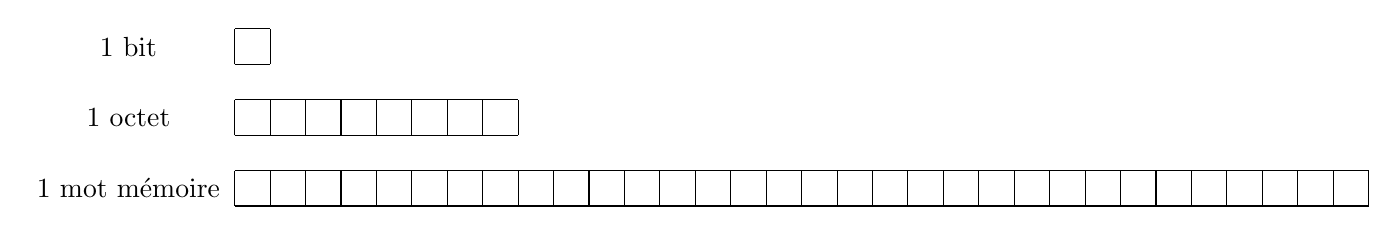
\begin{tikzpicture}[scale=0.45]
        \draw (0,0) grid (1,1); \node at (-3,0.5){1 bit};
        \draw (0,-2) grid (8,-1); \node at (-3,-1.5){1 octet};
        \draw (0,-4) grid (32,-3); \node at (-3,-3.5){1 mot mémoire};
    \end{tikzpicture}
    \captionof{figure}{Le bit est la plus petite unité informatique.}
\end{center}
\section{Encodage des entiers naturels}
\subsection{Écriture en base 10}
$$6103 = 6×10^3 + 1×10^2 + 0×10^1 + 3×10^0$$
\subsection{Écriture en base 2}
$$5 = 1×2^2 + 0×2^1 + 1×2^0$$
$$5_{10}=101_2$$
\subsection{Conversion}
\begin{center}
    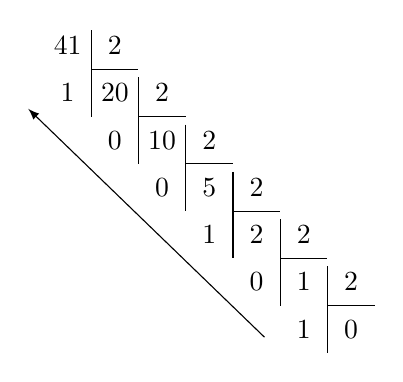
\begin{tikzpicture}
        \node at(0,0){41};
        \node at(0.6,0){2};
        \node at(0,-0.6){1};
        \node at(0.6,-0.6){20};
        \draw (0.3,0.2)--(0.3,-0.9);
        \draw (0.3,-0.3)--(0.9,-0.3);

        \node at(1.2,-0.6){2};
        \node at(0.6,-1.2){0};
        \node at(1.2,-1.2){10};
        \draw (0.9,-0.4)--(0.9,-1.5);
        \draw (0.9,-0.9)--(1.5,-0.9);

        \node at(1.8,-1.2){2};
        \node at(1.2,-1.8){0};
        \node at(1.8,-1.8){5};
        \draw (1.5,-1.0)--(1.5,-2.1);
        \draw (1.5,-1.5)--(2.1,-1.5);

        \node at(2.4,-1.8){2};
        \node at(1.8,-2.4){1};
        \node at(2.4,-2.4){2};
        \draw (2.1,-1.6)--(2.1,-2.7);
        \draw (2.1,-2.1)--(2.7,-2.1);

        \node at(3.0,-2.4){2};
        \node at(2.4,-3.0){0};
        \node at(3.0,-3.0){1};
        \draw (2.7,-2.2)--(2.7,-3.3);
        \draw (2.7,-2.7)--(3.3,-2.7);

        \node at(3.6,-3.0){2};
        \node at(3.0,-3.6){1};
        \node at(3.6,-3.6){0};
        \draw (3.3,-2.8)--(3.3,-3.9);
        \draw (3.3,-3.3)--(3.9,-3.3);
        \draw [->,>=latex] (2.5,-3.7) -- (-0.5,-0.8);
    \end{tikzpicture}
    \captionof{figure}{$41_{10}=101001_2$}
\end{center}
\subsection{Écriture en base 16}
La base 16 est régulièrement utilisé pour représenter les nombres binaires plus facilement. Chaque chiffre hexadécimal est représenté par 4 bits.
\begin{aretenir}[]
    1 octet est représenté par 2 chiffres hexadécimaux.
\end{aretenir}
\begin{center}
\begin{tabular}{|c|c|c|}
    \hline
    décimal & hexadécimal & bits \\
    \hline
    0       & 0           & 0000 \\
    \hline
    1       & 1           & 0001 \\
    \hline
    2       & 2           & 0010 \\
    \hline
    3       & 3           & 0011 \\
    \hline
    4       & 4           & 0100 \\
    \hline
    5       & 5           & 0101 \\
    \hline
    6       & 6           & 0110 \\
    \hline
    7       & 7           & 0111 \\
    \hline
    8       & 8           & 1000 \\
    \hline
    9       & 9           & 1001 \\
    \hline
    10      & A           & 1010 \\
    \hline
    11      & B           & 1011 \\
    \hline
    12      & C           & 1100 \\
    \hline
    13      & D           & 1101 \\
    \hline
    14      & E           & 1110 \\
    \hline
    15      & F           & 1111 \\
    \hline
\end{tabular}
\end{center}
\subsection{Python et les entiers}
\begin{itemize}
    \item Par défaut les nombres entiers sont encodés en base 10 en Python.
    \item Pour utiliser des nombres binaires, il suffit d'ajouter le préfixe \texttt{\textbf{0b}}.
    \item Le préfixe \texttt{\textbf{0x}} permet de manipuler des nombres en base hexadécimale.
    \item La fonction \texttt{\textbf{bin()}} convertit en base 2 n'importe quelle valeur.
\end{itemize}
\end{document}